\documentclass[a4paper]{article}
\usepackage[T1]{fontenc}
\usepackage{amsmath,amsfonts,amssymb}
\usepackage[11pt]{extsizes}
\usepackage{graphicx}
\usepackage[top=2.5cm,bottom=2.5cm,right=2.5cm,left=2.5cm]{geometry}
\setlength\parindent{0px}
\title{Rust Remote.Access.Trojan}
\author{Antoine MARTIN, Wesley EDE, Amad MOHAMMAD, Denis REMACLE}

\begin{document}
   \maketitle
   \newpage
   \section{Objectifs}
   \subsection{Besoin}
Nous souhaitons appréhender et mieux comprendre le fonctionnement d'un R.A.T (Remote Access Trojan), l'écriture d'une relation client-serveur ainsi que l'apprentissage du language Rust.\\
Pour cela, rien de mieux que de pratiquer le language dans ce type de contexte.
\bigskip
\\
Ce projet commun sera également une vitrine de notre compétence et pourrait nous permettre d'acquerir une plus grande crédibilité sur le long terme.\\
La solution sera donc publié en tant que logiciel libre une fois la soutenance passée et nous devrions par conséquent signaler le repository Github aux grands éditeurs de solutions de cybersecurité.
   \subsection{Notre Approche}
Nous allons procéder par équipes de deux : Amad / Denis (Serveur et payloads) et Wesley / Antoine (Client Windows et payloads).\\
Cette organisation s'explique du fait de la disparité de niveau en algorithmique et en programmation dans notre équipe et cela permettra aux plus faibles de suivre le mouvement et de suggérer du code sans casser le code actuel.
\bigskip
\\
Ça permettra également l'écriture progressive de la documentation technique de la solution.\\
Nous allons également réunir les deux équipes au moins une fois par semaine pour faire un état de l'avancement du projet.
\bigskip
\\
Nous allons donc mettre en place un architechture semblable à celle-ci : \\
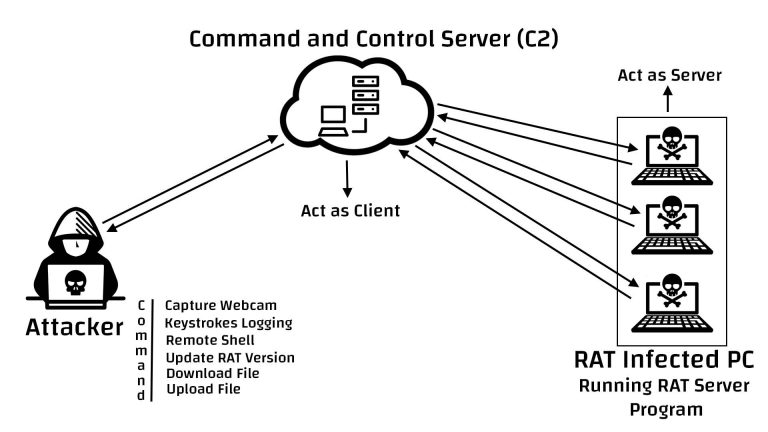
\includegraphics[scale=.5]{Schema.jpg}
\newpage
   \section{Planning}
Langage privilégié : Rust (Programme)\\
Langages scripts infection : Powershell
\bigskip
\\
En février nous aurons conceptualisé la relation client-serveur.\\
Le client compatible Windows pourra
 \begin{itemize}
\item "Contacter" le serveur (Connexion, extinction, heartbeat toute les heures)
\item Possibilité d'exécuter un reverse shell envoyé depuis le serveur
\end{itemize}
et le Serveur pourra :
 \begin{itemize}
\item Écouter sur un port et récupération de la liste des clients connectés
\item Gérer les differents clients (nommer, grouper, supprimer le client à distance)
\item Envoyer d'instruction au client (reverse shell)
\end{itemize}
\bigskip
Ensuite en avril, on aura ajouté différents payloads, en voici une liste qui seront mises en place :
 \begin{itemize}
\item Keylogger
\item Enregistrement du micro
\item Enregistrement de la caméra
\item Récupération des mots de passe sur navigateur
\item La connexion client serveur sera également chiffrée afin d'essayer de bypass certains firewalls.
\end{itemize}


Puis en Mai nous aurons commencer à travailler sur la mise en place d'une interface web pour la gestion du serveur avec les deux équipes en parallèle.
\newpage
\section{Etat des lieux des les solutions existantes}
Un RAT (Remote Administration Tool - Outil d'administration à distance) est un programme permettant la prise de contrôle totale, à distance, d'un ordinateur depuis un autre ordinateur.\\
Il est constitué de deux parties : le "client" et le "serveur". Le client est installé sur l'ordinateur de celui qui prend le contrôle et le serveur est installé sur l'ordinateur contrôlé.
\bigskip
\\
Il en existe de tout à fait légitime comme teamviewer ou le take control de N-Able RMM.\\
Mais il en existe aussi des malveillants comme nous allons le voir par la suite.
\bigskip
\\
Il existe divers Trojan RAT, un des plus anciens est BlackShades, le plus utilisé est Darkcomet ou NanoCore.\\
Ces chevaux de troie sont vendus mais on peut trouver des versions crackés, des tutoriels (dont des vidéos sur youtube) existent à foison.\\
Dès lors, n'importe qui, qui a très peu de connaissances peut se créer son propre Botnet (réseaux de PC infectés).
\bigskip
\\
Les RAT utilisent la relation "Client/Serveur" pour communiquer ;
\bigskip
\\
Premièrement on a un serveur sur lequel tourne l'instance malveillante chargée de centraliser les connexions. Plusieurs possibilités s'offrent à nous, on peut louer un serveur virtuel privé (type VPS) ou bien faire la faire tourner sur un ordinateur personnel, une VM etc.\\
Le serveur se présente sous la forme d'une interface qui permet de piloter les clients (machine infectée).\\
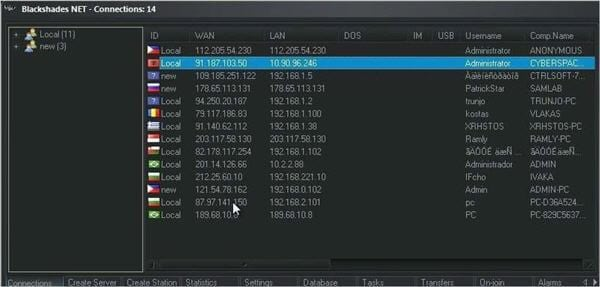
\includegraphics[scale=.5]{blackshades.jpeg}
\bigskip

Et une partie cliente (La cîble) qui se connecte au serveur : Le but est d'arriver à faire exécuter la partie cliente à l'insu de l'utilisateur afin de  prendre le contrôle de sa machine. La partie cliente est généralement très discrète voir transparente pour éviter d'éveiller les soupcons. En ce qui concerne les vecteurs d'attaque ils peuvent être multiples, par le biais notamment du social engineering puisque les personnes ciblées ne sont en général pas très férues d'informatique. L'attaque consistera en l'exécution d'un script de type "One-liner".
\newpage

\section{Le langage Rust}
Le Rust est un langage de programmation multi-paradigmes dont le développement a commencé en 2006 afin de créer un langage fiable, concurrent et pratique.\\
Ce langage s'appuie sur de nombreux conceptes 
\bigskip
\end{document}